

%----------------------------------------------------------------------------------------
%	PACKAGES AND DOCUMENT CONFIGURATIONS
%----------------------------------------------------------------------------------------

\documentclass{article}
\usepackage[english, italian]{babel}
\usepackage[T1]{fontenc}
\usepackage[utf8]{inputenc}
\usepackage{url}
\usepackage{graphicx}
\usepackage[hidelinks]{hyperref}
\usepackage{booktabs}

\setlength\parindent{0pt} % Removes all indentation from paragraphs

\renewcommand{\labelenumi}{\alph{enumi}.} % Make numbering in the enumerate environment by letter rather than number (e.g. section 6)

%\usepackage{times} % Uncomment to use the Times New Roman font

%----------------------------------------------------------------------------------------
%	DOCUMENT INFORMATION
%----------------------------------------------------------------------------------------

\title{Relazione Sito Web Populon \\ Progetto di Tecnologie Web} % Title

\begin{document}

\maketitle % Insert the title, author and date

\begin{center}
\textsc{\LARGE Componenti del gruppo:}\\[0.2cm]
 Diego Baratto \\ % Partner names
Mattia Biggeri \\
Paolo Bonato \\
Tommaso Padovan \\[0.2cm]
\textsc{\LARGE Referente:}\\[0.2cm]
 Mattia Biggeri\\
 biggeb4@gmail.com\\[0.2cm]
 \textsc{\LARGE Informazioni sul sito:}\\ [0.2cm]
http://tecnologie-web.studenti.math.unipd.it/tecweb/~mbiggeri/\\[0.2cm]
\textsc{\LARGE Informazioni di login}\\[0.2cm]

\begin{tabular}{l r} 
 Username: & admin\\
 Password: & admin\\
\end{tabular}\\[0.2cm]
\textbf{Anno accademico 2015/2016}
\end{center}

\newpage
\tableofcontents %Generazione indice
\newpage

 \newpage
%----------------------------------------------------------------------------------------
%	SECTION 1
%----------------------------------------------------------------------------------------

\section{Abstract}
	Il progetto consiste nella realizzazione di un sito internet basato su Populon, un gioco di ruolo ideato da uno dei
	componenti del gruppo assieme ad amici. Il sito ha lo scopo di far conoscere questo gioco e di aiutare a creare una comunità
	attorno ad esso e il gruppo ha quindi progettato il sito in quest'ottica. Le componenti essenziali scelte sono:
	\begin{itemize}
		\item Regole del gioco;
		\item Contenuti narrativi riguardanti il mondo di gioco;
		\item Possibilità di pubblicare notizie per gli utenti;
		\item Possibilità per gli utenti di condividere i personaggi da loro ideati.	
	\end{itemize}
	Queste componenti sono secondo il gruppo le più interessanti per gli utenti ma è stato lasciato spazio per future aggiunte.
	
%----------------------------------------------------------------------------------------
%	SECTION 2
%----------------------------------------------------------------------------------------

\section{Utenti destinatari}
	Il sito si propone a tutti gli utenti interessati ai giochi di ruolo. Siano essi dei curiosi inesperti o giocatori 
	abituali possono trovare facilmente tutte le informazioni che possono interessare. Inoltre il sito è pensato per gli
	utenti che già conoscono il gioco e sono interessati a notizie che lo riguardano e a condividere le loro avventure.

%----------------------------------------------------------------------------------------
%	SECTION 3
%----------------------------------------------------------------------------------------

\section{Accessibilità}

\subsection{Separazione tra contenuto, presentazione e struttura}
	Il sito è stato realizzato tenendo sempre ben separati contenuto, presentazione e struttura.
	Il codice HTML non contiene script nè impostazioni di stile, anche quando viene generato da funzioni in Perl.
	Tutte le regole di stile sono racchiuse all'interno di un unico file apposito.
	Le pagine che fanno uso di funzioni in Perl si trovano tutte in un'apposita cartella separata.
	Anche i file \texttt{.xml} e \texttt{.xsd} che formano il database sono separati dal resto del sito.
	In questo modo il sito è più facile da estendere e mantenere in quanto facile da comprendere.
	Inoltre queste attenzioni contribuiscono ad evitare la ripetizione di codice e a diminuire le dimensioni totali,
	velocizzando così le ricerche degli utenti.

\newpage
\subsection{Schema colori}

I colori utilizzati sono principalmente sui toni del blu, con un tono scuro per la struttura (header, footer e contorno) ed un azzurro molto più chiaro per lo sfondo ed il testo interno alle zone scure. La scelta di questi due colori è stata fatta per rendere il sito piuttosto gradevole alla vista senza affaticare gli occhi con colori molto brillanti senza però dimenticare la necessità di contrasti elevati per una buona comprensione del contenuto.
	Tutti i colori utilizzati sono considerati "WebSafe", quindi rappresentati con le stesse tonalità anche su monitor e browsers molto vecchi.
	L'accostamento di colori scelto risulta ad alto contrasto anche per persone affette da disturbi nella percezione dei colori, come dimostrato dagli screenshot di seguito, ottenuti grazie al programma gratuito ColorOracle. \\

\newpage	
	 \begin{figure}
				\centering
				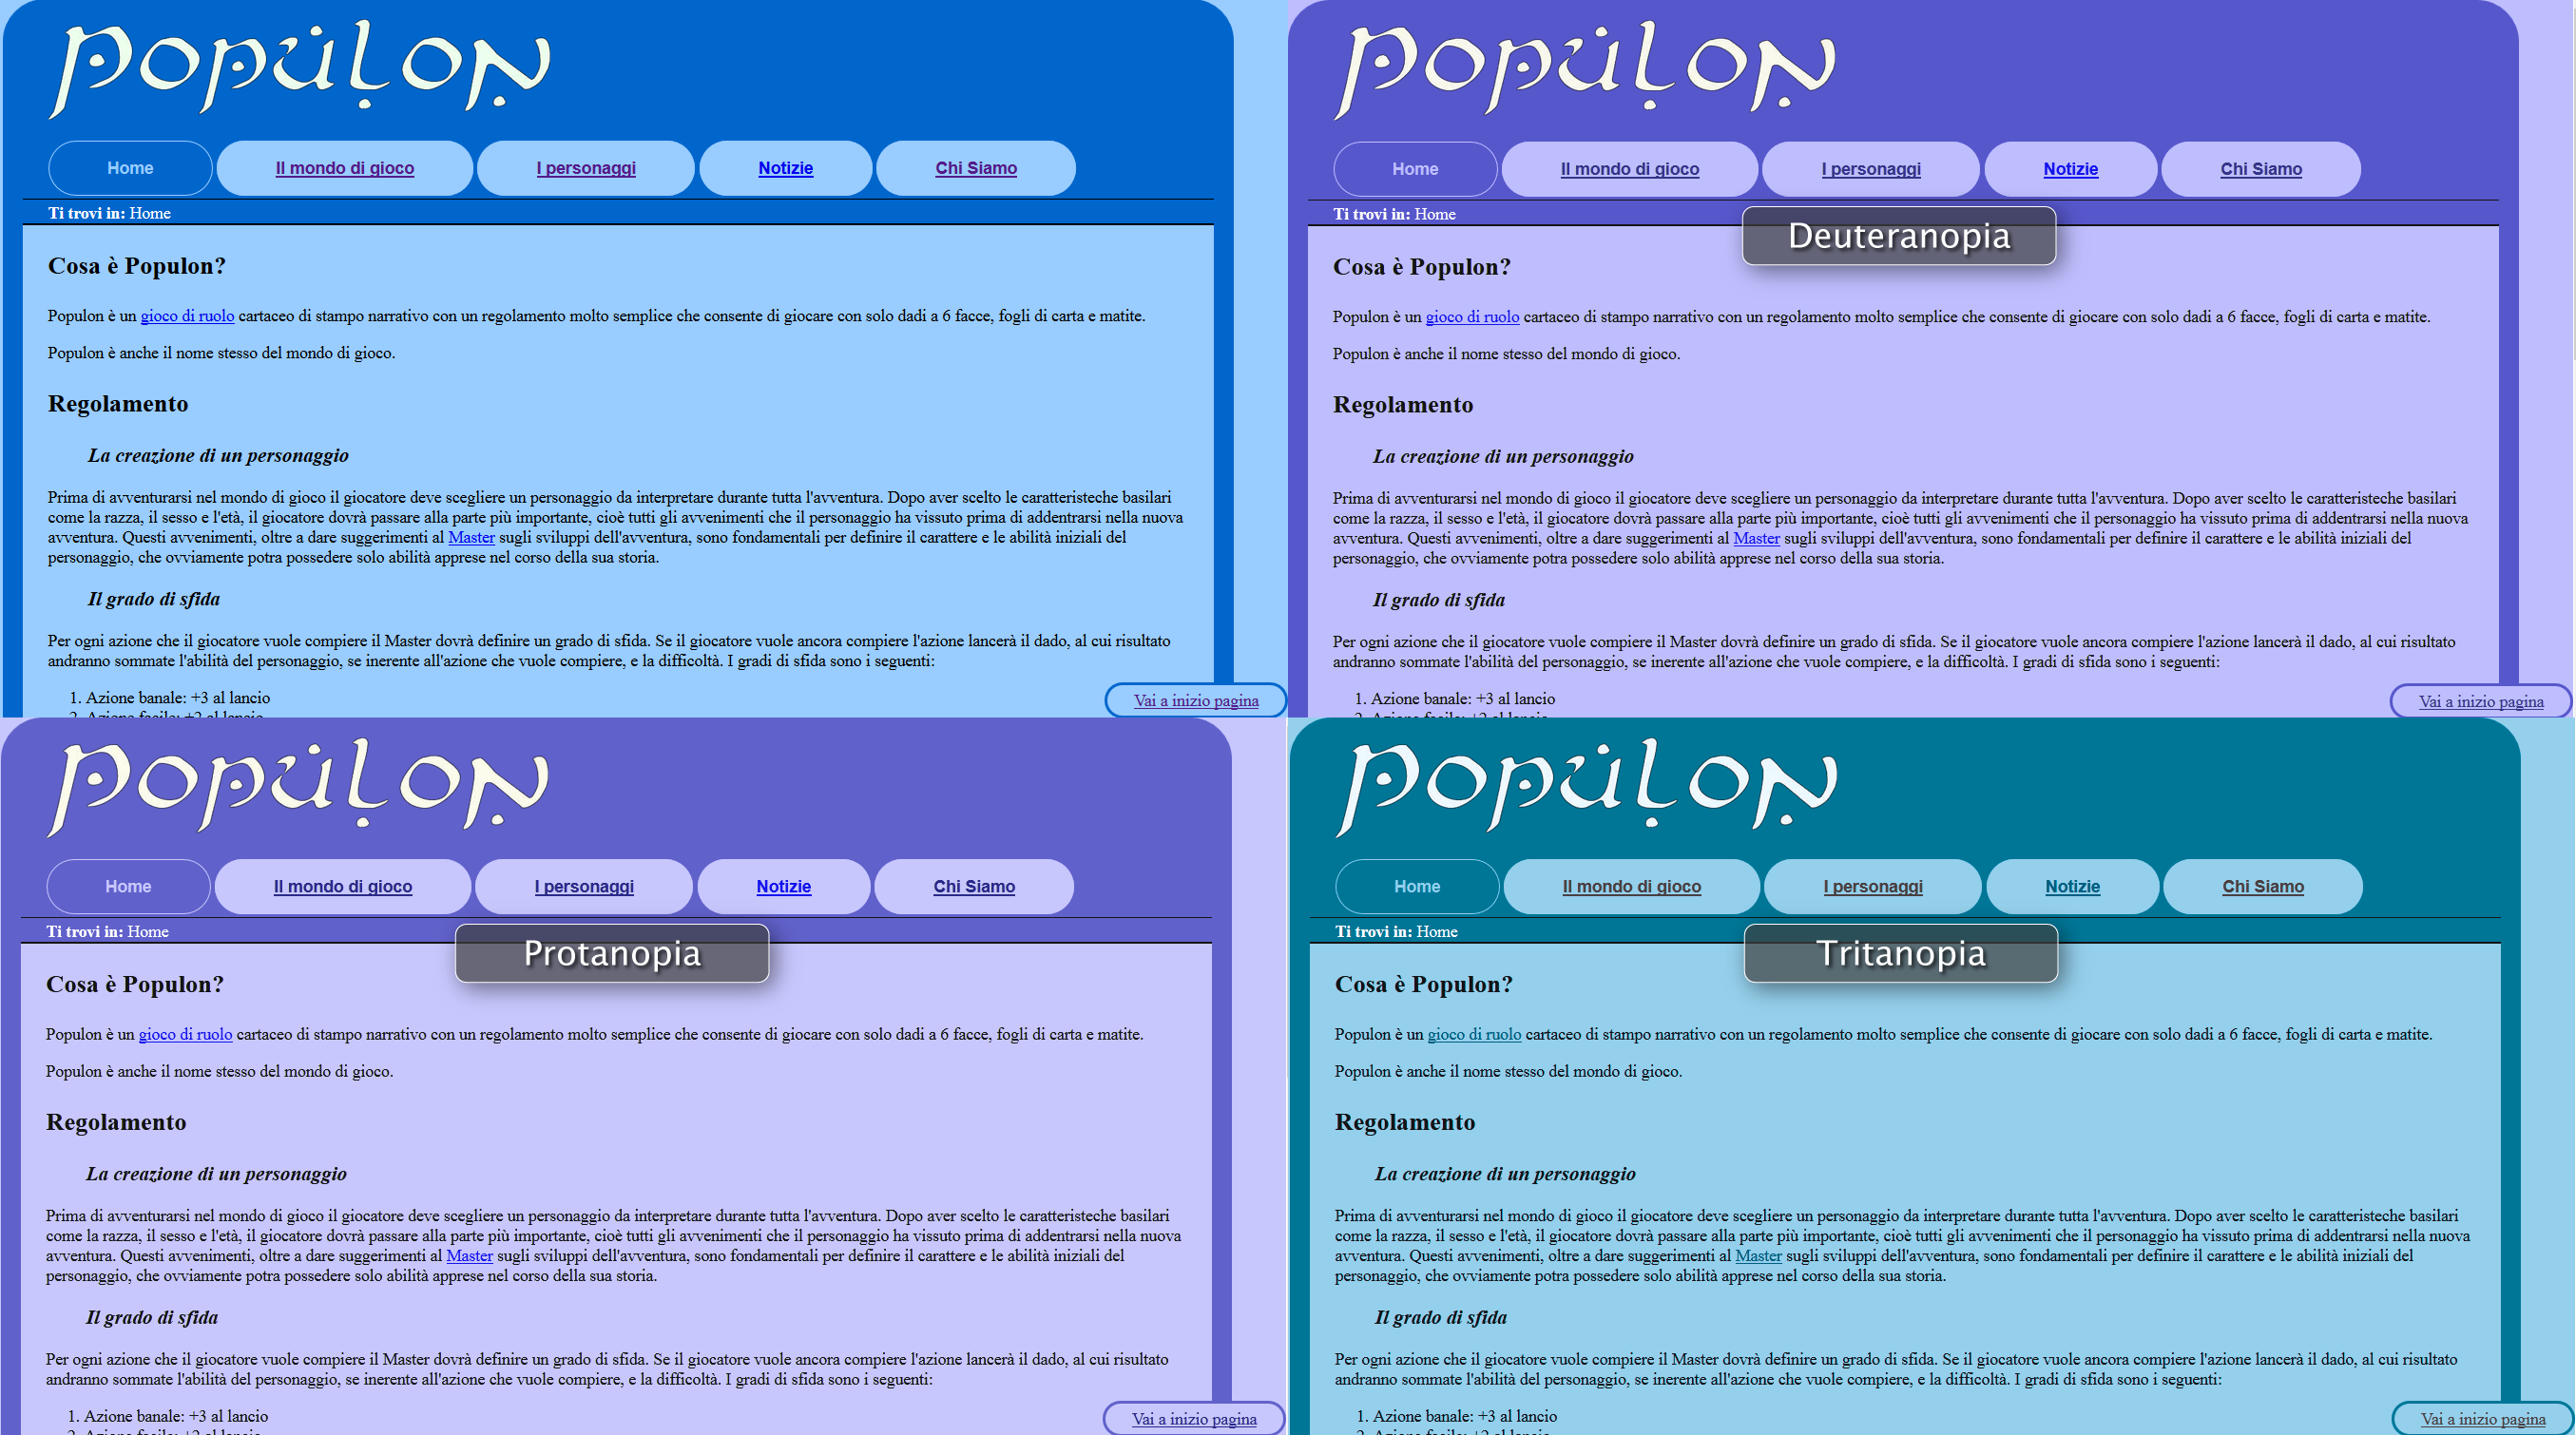
\includegraphics[scale=0.20]{all4.png}
				\caption{Percezione colori per le principali forme di daltonismo.}
			\end{figure}
			\newpage

\subsection{Tag meta}
	Sono stati inseriti per ogni pagina i tag meta: Content-Type, keywords, description, author e languages e il tag title, 
	il quale descrive la pagina corrente dal particolare al generale. 
	Il tag languages indica che il sito è stato interamente scritto in italiano ma compaiono alcune parole inglesi, 
	le quali sono state affiancate dall'attributo: xml:lang="en".

\subsection{Screen reader}
Tutte le immagini di contenuto possiedono attributi ALT e TITLE volti a spiegarne il soggetto nel modo più esaustivo possibile. Oltre a quelle non sono presenti altre immagini o altri oggetti in grado di ostacolare la fruizione del sito ad eventuali utenti non vedenti.

\subsection{Facilitazioni per la navigazione}
Sono stati presi provvedimenti volti a facilitare la fruizione del sito a utenti inabili:
		Link per saltare i menu: sono stati inseriti due link nascosti all'utenza normale ma visibili tramite screen reader che consentono di saltare i due menu presenti, quello di navigazione tra le sezioni del sito e quello interno alle spiegazioni del mondo di gioco;
		
		Link per tornare all'inizio: in ogni pagina è presente un link che consente di tornare all'inizio della pagina. Per gli utenti normovedenti, esso è stato collocato in posizione fissa in basso a destra nella pagina. Tale link è presente sia nella versione desktop che in quella mobile.


%----------------------------------------------------------------------------------------
%	SECTION 4
%----------------------------------------------------------------------------------------

\section{Usabilità}

\subsection{Le sei W}
La home page del sito si propone di rispettare la maggior parte dei sei assi informativi principali:
\begin{itemize}
\item \textbf{WHO:} Come da convenzioni del web design, il logo del sito è stato posto in alto a sinistra;
\item \textbf{WHERE e WHAT:} Il testo presente nella home page si prefigge lo scopo di spiegare ad nuovo utente di cosa tratti il sito e offre un'infarinatura di base sul regolamento del gioco di ruolo descritto. Inoltre sono presenti link a pagine esterne esplicative di determinati concetti che potrebbero non essere noti ai neofiti;
\item \textbf{WHEN:} Tale asse non è presente nella home page. Le sue funzioni di informazione sulle ultime novità sono state demandate alla pagina Notizie accessibile tramite la barra di navigazione; 
\item \textbf{HOW:} Tale asse è spezzato in due parti: la barra di navigazione illustra tutte le sezioni principali della pagina le quali, al loro interno, contengono collegamenti alle sezioni secondarie.
\end{itemize}

\subsection{Barra di navigazione}
 Viene sempre evidenziata la voce della barra di navigazione che indica la pagina corrente. Essa non è cliccabile, evitando così di ricaricare inutilmente la pagina. Inoltre quando una voce è puntata dal mouse viene evidenziata, suggerendo all’utente che può essere premuta, e questo non avviene per la pagina corrente.
	
\subsection{Breadcrumbs}
In ogni pagina, appena sotto la barra di navigazione, è presente il percorso che porta a quella pagina dalla relativa sezione principale del sito. Dato lo scarsissimo annidamento delle pagine, però, si raggiunge soltanto il secondo livello. I livelli precedenti a quello corrente sono presenti nella forma di link cliccabili, che riportano a quella pagina.
\subsection{Convenzioni e metafore visive}
Il sito rispetta alcune delle principali convenzioni visive in grado di aumentare l'usabilità:\newline
			I pulsanti della barra di navigazione sono colorati in modo diverso per evidenziare la sezione corrente. Inoltre, sono stati lasciati i link come da standard del browser, senza modificare l'aspetto dei link per lasciare un'idea di familiarità all'utente.\newline
			Inoltre, se ci si trova in una delle sezioni principali il corrispondente pulsante non è cliccabile.
			Le immagini risultano nitide anche su schermi di modeste dimensioni ed è possibile, volendo, visualizzarle a dimensione completa cliccandole col tasto destro del mouse e selezionando "Visualizza immagine" o tramite il metodo standard del long tap in ambiente mobile. Tale scelta è stata preferita al collegamento diretto per evitare eventuali aperture involontarie dovute a click inconsci sulle immagini, con conseguente confusione dell'utente.\newline
\subsection{Link}
I link utilizzati rispettano la colorazione tipica, compresa la colorazione differente una volta visitati. Inoltre il gruppo ha
posto attenzione a non utilizzare colori simili in altre parole del testo per evitare di confondere l'utente.


%----------------------------------------------------------------------------------------
%	SECTION 5
%----------------------------------------------------------------------------------------

\section{File}
\subsection{Gerarchia}
	I file sono stati organizzati tenendo le pagine HTML il file dei css e degli script nella cartella principale 
	\texttt{populon}. Al suo interno ci sono le cartelle: 
		\begin{itemize}
			\item \texttt{cgi-bin} che contiene tutte le pagine che fanno uso di funzioni in Perl;
			\item \texttt{database} che contiene tutti i file XML e i relativi schemi;
			\item \texttt{img} che contiene tutte le immagini del sito.
		\end{itemize}
\subsection{Struttura}

	Le pagine statiche sono state scritte rispettando lo standard XHTML 1.0 Strict e si trovano nella root folder del sito. Esse sono:\\
	
			\begin{itemize}
		\item Home.html: la home page del sito, contenente tutte le informazioni di base;\\
		\item IlMondoDiGioco.html: pagina contenente le informazioni principali sull'ambientazione del gioco di ruolo soggetto del sito.\\
		 Tale pagina contiene collegamenti a pagine interne in grado di descrivere meglio l'ambientazione:\\
		 \begin{itemize}
			\item artechnai.html\\
			\item eoyu.html\\
			\item glamordir.html\\
			\item miorning.html\\
			\item morte.html\\
			\item oros.html\\
			
		\end{itemize}
		\item Chi.html: contiene informazioni riguardanti i creatori del sito e qualche informazione sommaria sui creatori del gioco di ruolo.\\
		\item restricted.html: pagina di errore che compare se l'utente inserisce dati di login errati\\
		\end{itemize}

 \newpage
%----------------------------------------------------------------------------------------
%	SECTION 6
%----------------------------------------------------------------------------------------

\section{Presentazione}
	Per la presentazione grafica del sito è stato utilizzato lo standard CSS, arricchito da alcune funzioni proprie dello standard CSS3.\\ Tali funzioni riguardano principalmente l'arrotondamento dei bordi, la cui compatibilità con browsers più arretrati è stata aumentata tramite uso dei prefissi -webkit- e -moz-, e le media queries, utilizzate per determinare regole d'aspetto su dispositivi diversi dal normale PC quali smartphones o stampanti.\\
	Tutte le regole CSS sono contenute in un singolo file all'interno del quale si trova una suddivisione in "sezioni" determinata da commenti, onde facilitare eventuali modifiche o interventi mirati in caso di errori.\\
	

%----------------------------------------------------------------------------------------
%	SECTION 7
%----------------------------------------------------------------------------------------

\section{Comportamento}
	Perché il sito fosse più facile da utilizzare dagli utenti si è fatto un uso sostanzioso della tecnologia JavasScript, senza
	però renderla essenziale per il corretto funzionamento. La funzionalità più utile consiste nel controllo degli input delle 
	form. Il sito non accetta che vengano inseriti dati di tipo sbagliato o che ne manchino di obbligatori ma per fare questo è 
	costretto ad annullare l'operazione dell'utente. Grazie a JavaScript l'utente ha la conferma che i dati inseriti siano
	corretti prima di avviare la procedura. \\
	Nella form di inserimento di un nuovo personaggio sono messi a disposizione dell'utente ben 68 diversi dati in input di 
	cui solo 7 obbligatori e questo può disorientare l'utente. Grazie a JavaScript è stato possibile ridurre i campi visibili
	a 14 con la possibilità di aggiungerne alla necessità.

%----------------------------------------------------------------------------------------
%	SECTION 8
%----------------------------------------------------------------------------------------

\section{Gestione dei dati}
	\subsection{XML}
		Il sito necessita di tre tipologie di dati:
		\begin{itemize}
			\item \textbf{Amministratore: } Rappresenta un amministratore del sito tramite uno username ed una password.
			\item \textbf{Novità: } Rappresenta una novità che un amministratore può scrivere e pubblicare nella pagina apposita.
				Consiste come minimo di una frase come titolo e offre vari campi facoltativi tra cui data, ora, luogo e
				descrizione. Ogni notizia è identificata da un ID univoco.
			\item \textbf{Personaggio: } Rappresenta un personaggio del gioco inventato da un utente. Ha una struttura complessa 
				che rappresenta al meglio il personaggio. I dati obbligatori sono: Nome, Razza, Età, Punti Corpo, Punti Mente, 
				Punti Spirito. I dati ulteriori invece comprendono un numero arbitrario di abilità per ogni 
				tipo(Corpo,Mente,Spirito) e una biografia del personaggio. Ogni abilità ha un suo Nome ed un suo Livello.
				Ogni personaggio è identificato da un ID univoco.
	\end{itemize}
	
	\subsection{XSD}
		Per verificare la validità dei dati sono stati creati degli appositi schemi che definiscono i vari tag che possono
		comparire nei file XML e quali sono gli elementi e gli attributi obbligatori.
		
	\subsection{XSLT}
		Inizialmente era stato ipotizzato di utilizzare dei fogli di trasformazione per visualizzare le notizie ma l'idea 
		è stata successivamente abbandonata per favorire delle ricerche più mirate e facili per l'utente.

%----------------------------------------------------------------------------------------
%	SECTION 9
%----------------------------------------------------------------------------------------

\section{Perl}
	Perl viene usato per gestire la visualizzazione e la gestione delle informazioni dinamiche. 
	Tali pagine assumono un comportamento differente se a visitarle è un amministratore.
	\subsection{Pagine Utente}
		Un utente ha a disposizione le seguenti pagine:
		\begin{itemize}
			\item \texttt{Notizie.cgi : } Pagina dove l'utente può consultare le notizie pubblicate.
				Le notizie vengono divise in gruppi di dieci dalle più recenti alle più datate.
				Questa pagina offre inoltre una funzione che filtra le notizie secondo tre parametri:
				il titolo deve contenere una data stringa,
				il luogo deve contenere una data stringa,
				la data deve corrispondere ad una determinata data.
				Le notizie appaiono solo come titolo e data ed espongono un link per visualizzarne i dettagli.
				
			\item \texttt{dettagliNotizia.cgi : } Pagina dove l'utente può visualizzare tutti i campi di una singola notizia.
			\item \texttt{personaggi.cgi : } Pagina dove l'utente può consultare i personaggi pubblicati.
				I personaggi vengono divisi in gruppi di dieci dai più recenti ai più datati.
				Questa pagina offre inoltre una funzione che filtra i personaggi secondo due parametri:
				il nome deve contenere una data stringa,
				la razza deve corrispondere ad una scelta.
				I personaggi appaiono come Nome e Razza ed espongono un link per visualizzarne i dettagli. 
			\item \texttt{dettagliPersonaggio.cgi : } Pagina dove l'utente può visualizzare tutti i dati relativi al personaggio selezionato.
			\item \texttt{aggiungiPersonaggio.cgi : } Pagina dove l'utente può compilare la scheda di un personaggio.
				Per la compilazione la pagina si avvale di un form che vincola il numero di abilità di un personaggio ad un
				massimo di dieci per ogni tipologia. La conferma invia i dati alla pagina \texttt{inserimentoPersonaggio.cgi}.
			\item \texttt{inserimentoPersonaggio.cgi : } Questa pagina svolge la funzione di inserire il personaggio appena
				creato dall'utente nel database. In assenza di JavaScript controlla che tutti i dati obbligatori siano presenti 
				e che corrispondano alla giusta tipologia. Infine la pagina mostra all'utente l'esito dell'operazione e fornisce 
				un pulsante per tornare alla pagina dei personaggi.
		\end{itemize}
		Se un utente tenta di accedere ad una pagina amministratore viene reindirizzato alla pagina \texttt{restricted.html}.
\subsection{Pagine Amministratore}
		Un amministratore ha a disposizione tutte le pagine utente e poche altre:
		\begin{itemize}
			\item \texttt{login.cgi : } Pagina che chiama la funzione di login per amministratori. Dopo aver controllato i dati
				mostra all'utente l'esito dell'operazione.
			\item \texttt{logout.cgi : } Pagina che chiama la funzione di logout per amministratori. Dopo aver eseguito la 
				funzione mostra all'utente l'esito dell'operazione.
			\item \texttt{Notizie.cgi : } La pagina risulta uguale alla pagina utente con la differenza che sono presenti su 
				ogni notizia i link alle pagine per la modifica e la cancellazione della notizia. 
				Inoltre è disponibile la funzione per scrivere una nuova notizia.				
			\item \texttt{dettagliNotizia.cgi : } Questa pagina mostra all'amministratore tutti i campi della notizia in
				 dettaglio ma a differenza della pagina per l'utente permette di modificarli.
				 Per la modifica la pagina si avvale di un form e la conferma invia i dati alla pagina 
				\texttt{inserimentoNotizia.cgi}.
			\item \texttt{scriviNotizia.cgi : } Pagina dove l'amministratore può aggiungere una nuova notizia.
				Per la compilazione la pagina si avvale di un form e la conferma invia i dati alla pagina 
				\texttt{inserimentoNotizia.cgi}.
			\item \texttt{inserimentoNotizia.cgi : } Questa pagina svolge la funzione di inserire la notizia appena
				creata dall'amministratore nel database. In assenza di JavaScript controlla che il titolo sia presente
				e che i dati corrispondano alla giusta tipologia. Infine la pagina mostra all'amministratore l'esito 
				dell'operazione e fornisce un pulsante per tornare alla pagina delle notizie.
			\item \texttt{processDeleteNotizia.cgi : } Pagina che chiama la funzione di eliminazione di una notizia dal
				database. Dopo aver eseguito la funzione mostra l'esito all'amministratore.
			\item \texttt{personaggi.cgi : } Stessa pagina dell'utente, con la sola aggiunta di poter eliminare un personaggio.
			\item \texttt{dettagliPersonaggio.cgi : } Stessa pagina dell'utente.
			\item \texttt{aggiungiPersonaggio.cgi : } Stessa pagina dell'utente.
			\item \texttt{inserimentoPersonaggio.cgi : } Stessa pagina dell'utente.
			\item \texttt{processDeletePersonaggio.cgi : } Pagina che chiama la funzione di eliminazione di un personaggio dal
				database. Dopo aver eseguito la funzione mostra l'esito all'amministratore.
		\end{itemize}			
	\subsection{Funzioni}
		La maggior parte delle funzioni sono state racchiuse nel file \texttt{funzioni.pl} per semplificare la scrittura degli 
		altri file ed evitare le ripetizioni di codice.
	\subsection{Sessioni}
		Solo gli amministratori fanno uso delle sessioni. Al momento del login se le credenziali sono corrette viene creata una
		sessione. Inoltre viene anche inviato un cookie all'amministratore, contenente l'id della sessione. Quindi ad ogni
		richiesta l'amministratore invia il codice della sessione e si controlla che questo esista.

%----------------------------------------------------------------------------------------
%	SECTION 10
%----------------------------------------------------------------------------------------

\section{Test e validazione}

	Per garantire che il sito sia correttamente visualizzato e che rimanga accessibile sul maggior numero di browser possibili 
	si è verificata la validità di tutte le pagine,sia quelle statiche che quelle generate dal Perl, e sono stati effettuati 
	dei test di visualizzazione su browser meno recenti. \\
	Per la validazione il gruppo ha utilizzato lo strumento Total Validator, impostato per verificare che le pagine rispettassero
	lo standard texbf{XHTML 1.0 strict}. Tutte le pagine che compongono il sito sono state sottoposte alla verifica e sono 
	risultate approvate.
	
	Il sito è stato testato sui seguenti browser:
	\begin{itemize}
		\item Mozilla; 
		\item Edge;
		\item Internet Explorer 8-9-10-11;
		\item Edge Windows 10 mobile;
		\item Chrome
		\item Opera
		\item Safari
		\item Edge - Xbox One
	\end{itemize}
	


 \newpage

%----------------------------------------------------------------------------------------
%	APPENDIX
%----------------------------------------------------------------------------------------

\appendix
	\section{Organizzazione del lavoro}
	
	\textbf{Diego Baratto:}\\
	\begin{itemize}
	\item Scrittura del file CSS
	\item Adattamento delle pagine statiche e dinamiche
	\item Stesura di parte della relazione
	\end{itemize}
\textbf{Mattia Biggeri:}\\
	\begin{itemize}
	\item Scrittura delle pagine statiche
	\item Validazione e correzione del codice
	\item Recupero delle informazioni per il contenuto
	\end{itemize}
\textbf{Paolo Bonato:}\\
	\begin{itemize}
	\item Scrittura dei file XML e XMLSchema
	\item Scrittura di parte delle pagine dinamiche in Perl
	\item Stesura di parte della relazione
	\end{itemize}
\textbf{Tommaso Padovan:}\\
	\begin{itemize}
	\item Scrittura di parte delle pagine dinamiche in Perl
	\item Scrittura degli script in JavaScript
	\end{itemize}
%----------------------------------------------------------------------------------------


\end{document}
\ No newline at end of file